% Diagram of Android activity life cycle
% Author: Pavel Seda 
\documentclass[border=10pt]{standalone}
\usepackage{tikz}
\usetikzlibrary{arrows.meta,arrows}
\usetikzlibrary{calc,decorations.markings}

\tikzset{%
  >={Latex[width=2mm,length=2mm]},
  % Specifications for style of nodes:
            base/.style = {rectangle, draw=black,
                           minimum width=4cm, minimum height=1cm,
                           text centered},
  fmu/.style = {rectangle, draw=black,fill=blue!30,
                           minimum width=3cm, minimum height=1.5cm,text height=-0.80cm},
       model/.style = {rectangle, draw=black,fill=red!30,minimum width=1.5cm,minimum height=0.5cm},
    solver/.style = {rectangle, draw=black,fill=green!30,minimum width=2cm, minimum height=1cm},
         tool/.style = {rectangle, draw=black, fill=orange!15,
                          minimum width=12cm, minimum height=3cm,text height=-1.00cm},
}
\begin{document}    
% Drawing part, node distance is 1.5 cm and every node
% is prefilled with white background
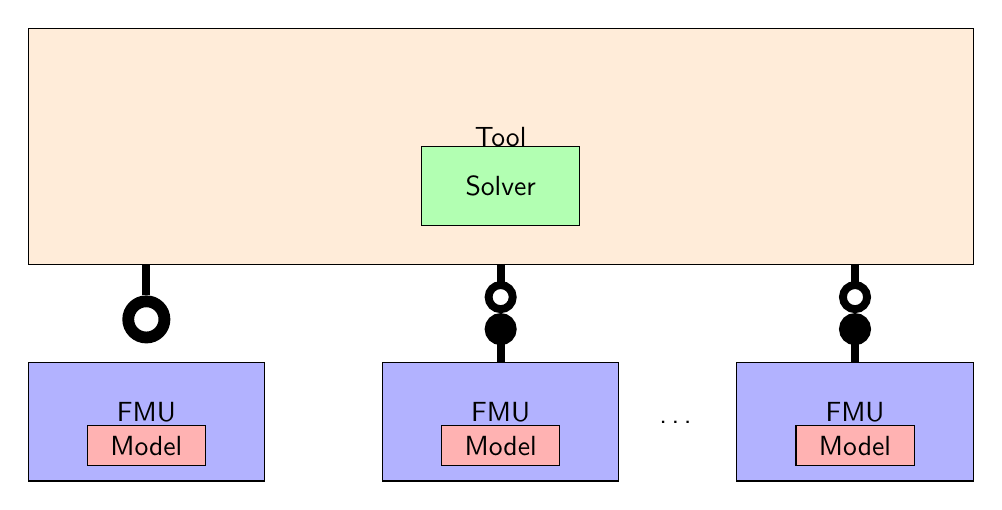
\begin{tikzpicture}[node distance=1.5cm,
    every node/.style={fill=white, font=\sffamily}, align=center]
  % Specification of nodes (position, etc.)
  
  
  \node (fmu1) [fmu] {FMU};
  \node (fmu2)  [fmu, right of=fmu1, xshift=3cm] {FMU};
	
	\node (fmu3)  [fmu, right of=fmu2, xshift=3cm] {FMU};
	
	\node (tool) [tool, above of=fmu2, yshift=2cm] {Tool} ;
	
	\node (solver) [solver, above of=fmu2, yshift=1.5cm] {Solver} ;
	
	\node (model1) [model, below of=fmu1, yshift=1.2cm] {Model} ;
	\node (model2) [model, below of=fmu2, yshift=1.2cm] {Model} ;
	\node (model3) [model, below of=fmu3, yshift=1.2cm] {Model} ;
	
  %\node (white1) [rectangle,above of=fmu1, yshift=0.625cm,minimum width=0.5cm,minimum height=0.5cm]
     
  % Specification of lines between nodes specified above
  % with aditional nodes for description 
\path (fmu2) -- node[auto=false]{\ldots} (fmu3);
%\draw[-*,line width=1.0mm] (fmu1) -- ([yshift=0.625cm]fmu1.north); 
\draw[-*,line width=1.0mm] (fmu2) -- ([yshift=0.625cm]fmu2.north);
\draw[-*,line width=1.0mm] (fmu3) -- ([yshift=0.625cm]fmu3.north);

\draw[line width=1.0mm,decoration={markings,mark=at position 0 with
    {\arrow[scale=1.5,>=stealth]{o}}},postaction={decorate}] ([yshift=0.85cm]fmu1.north) -- ++(0,0.4); 
\draw[-o,line width=1.0mm] ([yshift=1.25cm]fmu2.north) -- ++(0,-0.625);
\draw[-o,line width=1.0mm] ([yshift=1.25cm]fmu3.north) -- ++(0,-0.625);


  \end{tikzpicture}
\end{document}